\chapter{The Family Structure of Populations}
\label{cha:Lush_Chapter_24}
\index{Family differences|(}

Even in populations which are breeding entirely at random, an
individual does not have the same probability of being like every other
individual. Each is more closely related\index{Relationship} to some than to others. This
gives the population some kind of a family structure. Biological populations
are not as homogeneous as a population of balls or numbered
tickets in an urn, such as are often used to illustrate the elementary
laws of probability.

The definition of family always has in it something of the idea that
members of the same family are like each other and different from
members of other families. Yet usage varies widely as to the degree of
relationship which is meant. Sometimes family means a set of full sibs.
This is frequent in poultry breeding, but so restricted a definition is
uncommon in other animals where the number of full sibs is usually too
small for this to be very useful. In plants which can be self-fertilized,
family often means all the progeny of a single plant. It may mean a
more highly inbred group than that, but usually ``line'' is then used
rather than family. In animals which have long been linebred to a certain
individual, family may mean the whole group of individuals which
are linebred enough to be closely related to this individual and to each
other. An example is the Owl-Interest family of Jerseys.

In animals where little or no linebreeding has been practiced, family
is more likely to mean the descendants of a particular individual,
usually a purchased one (a ``foundation'' aimal [\textit{sic}]) or one thought to be
unusually good and with offspring well above average. Sometimes this
usage is carried to extremes, the family name being traced back only
through the female line (Shorthorns and Aberdeen-Angus) or only
through the male line (Herefords) to an ancestor so remote that, if there
has been no subsequent linebreeding, most of its descendants are little
if any more related to each other than they are to other animals of that
breed. Such usage is much like the transmission of family names in
man. There is little more reason to expect any real average difference
between Blackbirds and Ericas in Aberdeen-Angus than there is to
expect differences between the Smiths and the Wilsons in the United
States or between the Hansens and the Larsens in Denmark! The idea
of relationship between members of the same family becomes very dim
here, and family names tend to become artificial designations which
may be convenient but do not correspond to any biological reality.

Taxonomists use family in a special and definite sense to denote a
group which is intermediate between a genus and an order, as the cat
family (\textit{Felidae}), the deer family (\textit{Cervidae}), cattle
family (\textit{Bovidae}), etc.

We will consider first some of the less definite usages of family and
then the family as a basis for selection.

\section*{THE FAMILY --- A GROUP OF CLOSE RELATIVES}
\index{Family name|(}

When we say that an individual is from a good family, we usually
mean that the average merit of all its near relatives, regardless of whether
they are related through the sire or dam or bear the same family
name, is considerably above the breed average. This is the same sense in
which the term is often used in man when someone is said to be of ``a
good family'' or from ``a shiftless family.'' Family, in this sense of the
word, usually does not extend much farther among the collateral relatives
than to first cousins. Not often is anything implied about ancestors
farther back than the great grandparents, or about descendants much
more distant than grandsons and granddaughters. This use of family is
a practical application of relationship in estimating the heredity of an
individual from the appearance and performance of a considerable
number of its close relatives.

The family in this sense is somewhat indefinite, and one family
grades into another. For example, an individual's maternal uncles and
its paternal uncles are members of its family but the paternal uncles
need not belong to the family of the maternal uncles at all. In fact, no
two individuals would belong to exactly the same family unless they
were full sibs. The individual is at the center of its family with its relatives
clustered around it at various distances according to their relationship.
There is no accurate and simple formula for giving proper weight
to different relatives when averaging their good and bad qualities to
find the merit of the family, although of course the closest relatives are
the most important-unless there are strong environmental correlations
between them, as may sometimes be the case with maternal sibs. If the
family contains only a few members, chance can still play a large part
in giving one such family a good rating and another one a poor rating.

\section*{THE FAMILY NAME}

An Aberdeen-Angus cow is called an Erica if she traces through an
unbroken female line to the cow called Erica, regarded as the foundress
of the family. Technically she is still an Erica even if she does not trace
to Erica through any other line of her pedigree. In the Shorthorn and
Aberdeen-Angus breeds the family name is traced through the dams.
In the Hereford breed the family name is from the sire. In most dairy
breeds the family name comes from the dam, but in some both systems
prevail. The Holstein-Friesians have the De Kol family and the Pietertje
family which take their names from foundation cows, but the
Netherland family takes its name from the bull. In the Jersey breed
such families as Tormentor and Golden Lad are named after bulls; but
there are also such families as Coomassie, Fontaine, and Oxford named
after cows. Breeders of cattle and horses mention family more than do
breeders of sheep and swine.

This idea of family is a natural development in one-sire herds. A
breeder with several cows but only one bull will, of course, observe
many differences between his calves. Since all his calves in any one calf
crop are sired by one bull, it would be natural to assume, without even
realizing that he had done so, that all the differences between the calves
were due to differences in their dams. If when the successive calves from
the same cows are compared it is seen that there is a general tendency
for one cow to have good calves and another one to have mediocre
calves, it is natural for the breeder to group his animals in his own mind
in terms of their dams or grandams, as far back as he remembers those.
The inference that all the differences between the calves are due to differences
in their dams is, of course, unjustified, since the sire is never
entirely homozygous and some of the differences between the calves
will be due to difference in the inheritance they have received from him.
This tendency for the owners of small herds to think of families in
terms of female foundation animals is reversed in large herds where
several sires are maintained at all times. It is difficult for the breeder to
know all of his individuals closely in such herds and easy for him to
compare the calves by one sire with their contemporaries by other sires.
This naturally leads to a system of referring to the calves in terms of
their sires and grandsires instead of their dams. Perhaps this is responsible
for the fact that the Hereford breed, which is prevailingly bred in
large herds, tends to trace its family through the male line, whereas
breeds more commonly bred in small herds tend to trace the family
through the dam.

\index{Pedigrees, abbreviated|(}
When the system of tracing the family name through the dam is followed
far, it naturally leads to printing the pedigrees in the ``abbreviated''
form, a sample of which is shown herewith in the pedigree of the
noted Shorthorn bull, Rodney. Pedigrees in cattle breeds other than
the Shorthorn are now usually printed in the bracketed form which
gives information on all lines to the same number of generations.
Breeders of horses often use the abbreviated pedigrees. Formerly only
that part of the pedigree which appears in columns in this example was
shown. In recent years footnotes about the three most recent sires are
added, as in this case. Figure 42 shows the pedigree as it would appear
in bracketed form. The line drawn across the pedigree separates the
information which is contained in the footnotes from that which is
given in the columns.

\begin{figure}
	\centering
    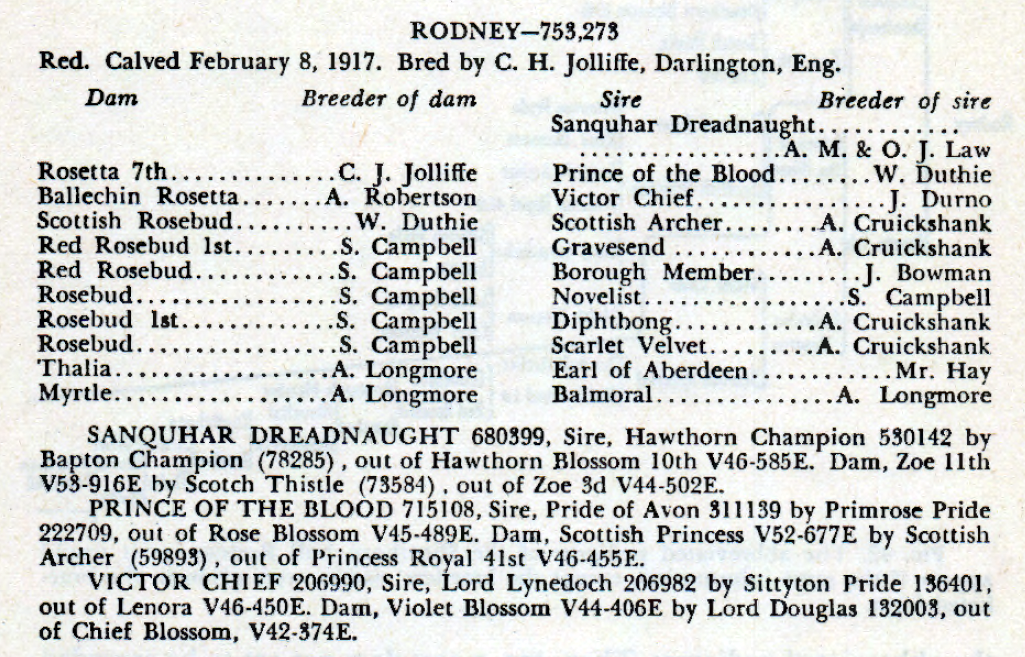
\includegraphics[width=\textwidth]{Page_311.png}
    \label{fig:Lush_Figure_Page_311}
\end{figure}

\nowidow
This abbreviated form of pedigree was fairly adequate when all of
the breeders were acquainted with the sires which were being used in
the prominent herds. There was no need to print the pedigree of the
sire, since each potential customer knew that. The customer would not
know all the females of the breed, so he did want to see the pedigrees of
the cows. When the breeds grew larger the time came when no one
knew all the sires; therefore, it became necessary to add these footnotes.
The abbreviated pedigrees emphasize remote ancestors beyond all usefulness.
For example, Rodney is called a member of the ``Rosebud family''
after the cow, Rosebud (by Scarlet Velvet), which was the first one
bred by S. Campbell, who developed this family. If there has been no
linebreeding to Rosebud in Rodney's pedigree, his relationship to her
will be \(\nicefrac{1}{2}^8\), which is about 0.4 per cent of his genes which probably
came from her. Rodney must have had literally tens of thousands of
contemporary relatives which had other family names but were more
closely related to him than was the cow from which his family name
comes.

The abbreviated pedigrees emphasize the names of the breeders.
The value of any pedigree is affected by the general reputation of the
herd in which the animal was bred. Something worth while is lost when
the name of the breeder is given a less prominent place than it has in
the abbreviated pedigrees. Then, too, a cow does not get to be regarded
as the foundress of a family on her own merits alone, but rather on the
high merit of many of her offspring. It is fairly safe to infer that Rosebud
1st and also Rosebud (by Novelist) were distinctly better individuals
than average or else Rosebud (by Scarlet Velvet) would not have
been regarded as the foundress of a family.

\begin{figure}
	\centering
    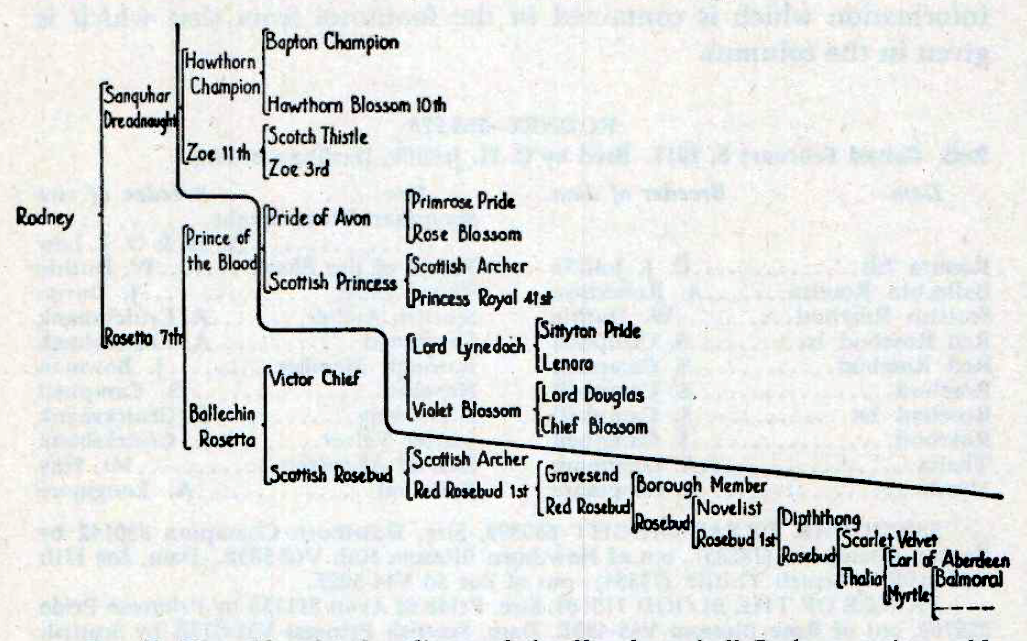
\includegraphics[width=\textwidth]{Figure_42.png}
    \caption{The abbreviated pedigree of the Shorthorn bu11 Rodney, as it would
			 appear if the same information, except the breeders' names, were
			 given in the bracketed form.}
    \label{fig:Lush_Figure_42}
\end{figure}

\index{Pedigrees, abbreviated|)}
The commercial importance of the family name is usually small,
unless perhaps in times of booms or pedigree speculation. It lends itself
well to speculation, particularly in breeds where the family name is
traced only through the female line. Even the best of cattle are none
too prolific, and a family can become famous and remain famous for
many years without a large number of females of that family ever existing
at any one time. If a strong demand for a family name can be created,
extreme speculation can easily result because the supply is limited.
Naturally such speculation is rare except when there is general prosperity
and prices for breeding stock have been rising for some time. The
most noted case of this kind was the speculation that went on in the
``pure'' Duchess Shorthorns in the 1870's. There have been several
periods of less extreme speculation in Aberdeen-Angus family names.
Yet in 21 Aberdeen-Angus sales, studied from this point of view from
1929 to 1938 in Iowa (unpublished), the only conclusion possible is that
practically no cash was really being paid for family name. However, this
was in a period of economic depression and perhaps this finding is not
significant. Four more sales from 1940 to 1942 when prices were rising
showed distinct price differences between families.

The family name has genetic importance when the animal which
gave its name to the family is still within three or four generations of
the animals concerned. In such a case the coefficient of relationship
between the animal and the foundation animal is still high enough to
mean that the two are apt to be alike in a noticeable proportion of
their genes.

Paying attention to maternal family names compels a certain
amount of added attention to the females in breeding selections. Some
breeders might be more careless about the dams if it were not for this
extra attention forced on them by the family system. The actual importance
of this may be slight.

The family name would have some genetic importance whenever
the general condition exists that breeders strive always to mate a cow of
one family to a bull of the same family; that is, to breed the family
``pure.'' If S. Campbell had always sought Rosebud bulls to mate to his
Rosebud cows, and if this had been continued to Rodney's time, Rodney
would have been kept very closely related (linebred) to the original
Rosebud cow. If that were a general practice among most breeders, it
would lead to steady linebreeding which might keep the foundation
animal important for many generations after its death. Where the family
system brings this about, it can be a powerful instrument in improving
the pure breeds, but this does not happen often. The cows in a small
herd may belong to a dozen families, but the same bull is usually mated
to all of them.
\index{Family name|)}

\section*{THE LINEBRED FAMILY}
\index{Linebreeding|(}

Sometimes ``family'' is used to designate a group which has been
partially separated from the rest of the breed for a long time in their
breeding and among which there has been considerable linebreeding.
Not often have such cases really been carried far enough to make the
family very distinct from the rest of the breed. Even a slight separation
of this kind has sometimes been the occasion for a large amount of
speculation in pedigrees. The most famous case is that of the ``pure''
Duchess Shorthorns, for which the pedigree speculation reached its
climax in 1876 in the New York Mills sale where one cow sold for
\$40,600. The ``pure Scotch'' Shorthorns are another example. In spite
of many bitter condemnations of the ``straight Scotch'' craze, the
straight Scotch almost entirely displaced the other beef Shorthorns in
the United States during the two decades preceding 1920. The ``straightbred''
or ``airtight'' Anxiety 4th Herefords may be a similar case in
which the final outcome is still in doubt. These straightbreds are a
group whose pedigrees in nearly every line go to daughters of North
Pole and to sons and daughters of Anxiety 4th. That is, they carry nearly
50 per cent of the blood of North Pole and Anxiety 4th combined.
Somewhat milder cases have happened in the Jersey breed in connection
with the Owl-Interests, the St. Lamberts, and Tormentors, and in
the Holstein-Friesians with the Homestead family.

The principles involved are just the same as those that have been
discussed under linebreeding. If the linebreeding has been carried far
enough to make the family really distinct from the rest of the breed,
then there is an important genetic basis for the family name. This kind
of a family is to some extent a breed within a breed.
\index{Linebreeding|)}

\section*{THE GENETIC DEFINITION OF FAMILY}
\index{Relationship|(}

The biological basis for treating a group as a family is the average
genetic likeness among members of the group. The best estimate of
genetic likeness where the actual genotypes are unknown is the coefficient
of relationship. This will usually give a reasonably true picture of
the average genetic likeness of family members where the base to which
relationship was computed is not many generations in the past.

As an example of this way of defining a family quantitatively, we
might choose to consider each set of full sibs in a random breeding
population as a family. For comparison with other kinds of families
we can define this kind as a group which are related to each other 50
per cent. If all the offspring of each male are to be considered as a family,
that kind of a family can be defined as a group related 25 per cent to
each other.\footnote{Although such a family will not be entirely homogeneous
if some of them are full sibs to each other, this will not increase the average
relationship much if there are more than three or four different sets of such
full sibs or if the number in each such set is small. For example, if the
progeny of a boar consist of four litters of five pigs each and we call this a
family, it will not of course be a perfectly homogeneous family but will be
one large family with four branches or subfamilies. The average relationship
of each pig to the other 19 will be an average of 4 full sib and 15 half sib
relationships or about 110 per cent. If the progeny of a bull are five pairs
of full sisters, the average relationship within the group of 10 will be an
average of 1 full sib and 8 half sib relationships or 28 per cent.} We can
compare the importance we should attach to family when making selections in
the two cases by using alternately .50 and .25 for \textit{r} in the formulas
which are in the next few pages. If all the grandsons and granddaughters of
a male are to be considered as a family, we can define this family as a group
which are related to each other 6\nicefrac{1}{4} per cent, plus a little
more from the fact that some of them will be sibs or cousins through more
than one grandparent. When family is thus defined quantitatively, it is easy
to see why the practical usefulness of family groupings becomes so small
when the group members are related only through ancestors as distant as
grandparents.

The observed family resemblance may be expressed either in tenns
of the correlation between members of the same family or in terms of
how much smaller the differences between members of the same family
are than the differences between members of different families. The
formula which relates the two is simply that the correlation between
members of the same family equals $\dfrac{V - B}{V}$ where \textit{V}
is the variance between individuals which belong to different families
and \textit{B} is the variance between individuals which belong to the
same family. $V - B$ is the variance caused by things which are alike
for all members of each family but may vary from one family to another.
$V - B$ might be wholly genetic in some cases but is likely also to
include some differences caused by common environment for family mates,
or by epistasis, or dominance.

The formulas showing quantitatively the advantages and disadvantages
of selection on a family basis are rather complex but they arc given
in the following sections because they are important guides for
estimating whether a plan for selecting on a family basis is likely to
increase progress sufficiently to be worth its costs.

\section*{CONDITIONS AFFECTING PROGRESS WHEN CHOOSING BETWEEN FAMILIES}
\index{Selection!on the family basis|(}

The formulas for comparing individual and family selection, when
the same percentage of the population must be culled in either case,
are expressed as follows for convenience:
\vspace{-0.2cm}
\begin{table}[h]
	\centering
	\begin{tabular}{R{1cm}L{11cm}}
		Let~$G$ & = the additively genetic variance between individuals. \\
		$E$ & = all other variance (largely environmental in most cases) which is random\\
			& with respect to family. \\
		$C$ & = the variance caused by whatever fraction of the environmental,\\
			& epistatic, and dominance deviations are alike for members of the\\
			& same family, but vary from one family to another. \\
		$r$ & = genetic relationship between members of the same family. \\
		$t$ & = phenotypic or observed correlation between members of same
family $=$ \\
			& $\dfrac{rG + C}{G + C + E}$. \\
		$n$ & = number of individuals in each family.
	\end{tabular}
\end{table}
\vspace{-0.6cm}
\begin{table}[h]
	\centering
	\begin{tabular}{R{1cm}L{11cm}}
	Then: & Variance between individuals from different families \(= E + G + C\) \\
		  & Variance between members of the same family \(= E + (1 - r)G\). \\
		  & Variance between actual family averages $=$ \\
		  & \hspace{2.5em}\(rG + C + \dfrac{1 - r)G}{n} + \dfrac{E}{n}\).
	\end{tabular}
\end{table}
\vspace{-0.2cm}

Having large numbers in the family permits the environmental differences
(\textit{E}) and the genetic differences between members of the same
family --- the $1 - r$ fraction of \textit{G} --- to cancel each other, so that the actually
observed differences between family averages tend toward $rG + C$,
which will be almost wholly genetic if \textit{C} is very small. When \textit{n} is small
a considerable part of the differences between the actually observed
averages of various families may still be due to the $E/n$ term which is
environmental and misleading.

The larger \textit{r} is, the more of the genetic variance (\textit{G}) will be between
families instead of within families. This will permit the family averages
to be farther apart, so that one can reach farther when selecting
between families when \textit{r} is large than when it is small. Also any
increases in \textit{r} will make a larger fraction of the observed differences
between family averages genetic, so that one selecting between family
averages will actually get a larger fraction of what he reaches for. To
have \textit{r} large is an important prerequisite for selection between families
to be very useful.
\index{Relationship|)}

When \textit{C} is large the heritability of differences between family averages
will be low, since that heritability tends toward $\dfrac{rG}{rG + C}$ as \textit{n}
becomes indefinitely large. Hence, with \textit{C} large many of the differences
between family averages will not be genetic, many mistakes will be
made in selecting between families, and only a small fraction of what is
reached for in family selection will actually be gained in the merit of
the offspring. The deceiving effects of \textit{C} do not diminish with increases
in \textit{n} as those of \textit{E} do. In the mammals, \textit{C} is especially
likely to be important when the family consists of maternal sibs.\footnote{Environmental
correlations between full sibs are also prominent in data on
man, especially in data pertaining to mental and social traits. Man's long infancy and
childhood and the wide differences from home to home in cultural environments and
parental precepts and examples give an unusual opportunity for such correlations
to develop in characteristics which are susceptible to much modification by such
influences.} \textit{C} is likely to be large
also in birds which hatch and brood their own young. Even in birds
hatched in incubators and reared apart from their dams, certain initial
environmental differences caused by the size of the egg may not be
wholly equalized before the birds are adult. In data collected from
many different farms, \textit{C} is often troublesomely large because environments
vary considerably from farm to farm, and in most cases each family
will have been raised wholly on one farm. In carefully planned
breeding experiments every effort will be made to reduce \textit{C} to zero by
controlling or randomizing the environment with respect to families.
Often that can be fairly well achieved for all of \textit{C} except the part due to
maternal environment and the part due to weather and to changes in
general environment from year to year in cases where the families are
not contemporary. But breeders when purchasing animals usually must
compare families kept in different herds. Then the best they can do to
eliminate \textit{C} is to observe the conditions under which each family is kept
and make allowances for the differences which they think these conditions
produced between families.

\section*{FAMILY SELECTION COMPARED WITH INDIVIDUAL SELECTION}

For clarity we will first consider what family selection would accomplish
if it were practiced by itself without any attention to individuality.
Figure~\ref{fig:Lush_Figure_43} will illustrate the difference between family selection
alone and selection on an individual basis. The data are 180-day weights
of four pigs in each of four litters. One-fourth are to be saved for breeding
purposes, and selection is for the heaviest weights. If selection is
wholly on a family (litter) basis, the selected pigs will be all four of
those in family 2, since that family has the highest average weight. Pig
\textit{E}, which has a low weight, will be selected along with the other three
because it is in the family with the high average. If selection is wholly
on an individual basis, pigs \textit{D}, \textit{G}, \textit{H}, and \textit{L},
will be selected regardless
of the merits of their sibs. If the method of selection is some compromise
which gives attention to family averages as well as to individual
merit, pigs \textit{F} and \textit{P} might possibly be saved instead of
pigs \textit{D} and \textit{L}.

Two things about this situation must be emphasized. First, one cannot
pay attention both to family apd to individuality without compromising
on both. Almost never will it happen that all members of the
family which has the highest average will be individually superior to all
members of the other families. One must compromise on one thing or
the other when deciding what to do with good individuals (like \textit{D} and
\textit{L}) from mediocre or poor families and with mediocre or poor individuals
(like \textit{F} and \textit{E}) from a good family. Second, some of the same animals
will be saved, no matter which method or compromise is used. The family
with the highest average must contain more than a fair share of individuals
which are above average. \textit{G} and \textit{H} illustrate this. Purely
individual selection does some of the same things which purely family
selection would do. If either method is \textit{absolutely} ineffective, the other
will be also. The contrast between them is between two methods both of
which will produce some improvement, if either of them will produce
any, but which will not, except by coincidence, produce exactly the
same amount of improvement per generation.

\begin{figure}
	\centering
    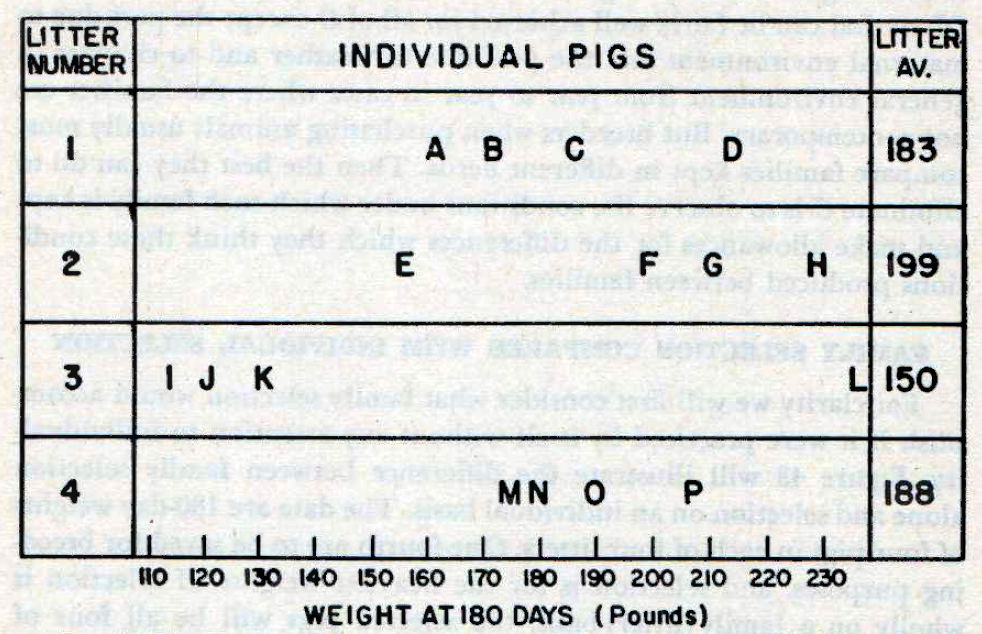
\includegraphics[width=\textwidth]{Figure_43.png}
    \caption{Distribution of some pig weights by litters to illustrate family and individual
			 selection. Each pig is designated by a letter located vertically according to its
			 litter and horizontally according to the pig's weight.}
    \label{fig:Lush_Figure_43}
\end{figure}

The increase in the population mean each generation under purely
family selection is expected to be the following fraction of the increase
to be expected under purely individual selection: \(\dfrac{1 + (n - 1)r}{\sqrt{n[1 + (n - 1)t]}}\).

Although this formula is complex, it can be seen that family selection
is most likely to be superior when \textit{r} is large and \textit{t} is small. Differences
in \textit{n} do not affect the ratio very much unless \textit{t} is extremely small
and \textit{r} is large. In that case high values of \textit{n} increase the effectiveness of
family selection markedly. If \textit{t} is nearly equal to \textit{r}, family selection can not
equal individual selection in effectiveness, even when \textit{r} and \textit{n} are
large.

\nowidow
If purely family selection is to produce improvement \textit{x} times as
rapid as would be produced by individual selection, then \textit{r} must equal
\(\dfrac{x\sqrt{n[1 + (n - 1)t]} - 1}{n - 1}\). For \textit{x} to be 1.0 when families
consist of 5, \textit{r} would have to be:

\begin{gather*}
.41 \text{ if } t \text{ is } .1 \\
.50 \text{ `` `` `` } .2 \\
.58 \text{ `` `` `` } .3 \\
.65 \text{ `` `` `` } .4 \\
etc.
\end{gather*}

If \textit{n} is as large as 25, the corresponding values of \textit{r} necessary
for \textit{x} to be l.O would be only a little lower, namely: .34, .46, .56, .64,
etc. In short, if family selection is to be much more effective than individual
selection, \textit{r} must be considerably larger than \textit{t}. Increases in
\textit{n} do not lower the requirements for \textit{r} much unless \textit{t} is very small.

Because \textit{t} equals $\dfrac{rG + C}{G + C + E}$, it is necessary for
\textit{C} to be nearly zero and \textit{E} to be much larger than \textit{G}
if \textit{r} is to be much larger than \textit{t}. When heritability is low
(\textit{G} is small, compared with $E + C$) neither
individual selection nor family selection will make rapid progress, but
family selection can then be considerably more effective than individual
selection if \textit{C} is zero or nearly so. Among important characteristics for
which \textit{E} is likely to be very large and \textit{C} may be small, are such complex
things as fertility, vitality, longevity, disease resistance in general,\footnote{Individual 
differences in resistance to some specific diseases may be rather highly genetic.} and
probably growth rate so far as that does not depend mainly on dimensions
of bones.

\section*{SUPPLEMENTING INDIVIDUAL SELECTION WITH FAMILY SELECTION}

It is sensible of course to use both the family average and the individual's
own characteristics in selecting, compromising somewhat on
each in order to make faster progress than could be made by using
either alone. The progress per generation which will be achieved under
the optimum combination of individual and family selection will be
the following fraction of what would be achieved by selection on individuality
alone:

\[ \sqrt{1 + \frac{(n - 1)(r - t)^2}{(1 - t)[1 + (n - 1)t]}} \]

The most important thing in determining how large this ratio will
be is the term, $r - t$, which measures how much more the members of
the same family are like each other genetically than they are outwardly.
When $t = r$, nothing at all is gained by paying attention to the family
average. The larger the difference between \textit{r} and \textit{t} the more there is to
gain by paying some attention to family. Even when \textit{t} exceeds \textit{r}, something
is to be gained from considering the family average, but in this
case the attention given to the family average is negative; i.e., the individual
is judged partly by its own merit and partly by how much it
deviates from its family average, instead of being given some credit if
the average merit of its family is high and being penalized if it is from a
poor family.

The numerical values in Table~\ref{tbl:Lush_Table_18} for some selected conditions may
make it easier to see what circumstances lead to much gain from paying
attention to family. The basic formula is that if paying attention both
to the individual and also to its family average is to make progress $1 + y$
times as rapid as if selection were on individuality alone, $r - t$ must
equal

\[ \frac{y(2 + y)(1 - t)[1 + (n - 1)t]}{n - 1} \]

\noindent
For progress to be made 20 per cent faster by considering the family
average requires the difference between \textit{r} and \textit{t} to be 1.45 times as large
as is necessary to increase progress by 10 per cent. If progress is to be
30 per cent faster, the difference between \textit{r} and \textit{t} will need to be 1.81
times as large; for 40 per cent it will need to be 2.14 times; for 50 per
cent 2.23 times is required; etc.

\begin{table}[htbp]
	\centering
	\caption{\textsc{Genetic Relationships Necessary if Paying Attention Also to Family is to
Iicrease the Rate of Improvement by 10 per Cent or by 100 per Cent}}
	\label{tbl:Lush_Table_18}
	\begin{tabular}{C{2cm}||C{2.25cm}|C{2.25cm}|C{2.25cm}|C{2.25cm}}
		\hline
		\hline
		 							& \multicolumn{2}{C{4.5cm}|}{For Progress to Be 10 per Cent
Faster (y = .1)}	& \multicolumn{2}{C{4.5cm}}{For Progress to Be Twice as Fast (y = 1.0)} \\
		\cline{2-5}
		t		& When $n = 5$ $r$~must $=$	& When $n = 25$ $r$~must $=$	& When $n = 5$ $r$~must $=$	& When $n = 25$ $r$~must $=$ \\
		\hline
		.01	& .27	& .11	& .89			& .40 \\
		.05	& .29	& .19	& .97			& .56 \\
		.10	& .36	& .26	& Impossible	& .72 \\
		.20	& .47	& .40 	& "				& .96 \\
		.30	& .58	& .52	& "				& Impossible \\
		.40	& .69	& .64	& "				& " \\
		.50	& .78	& .74	& "				& " \\
		.60	& .87	& .83	& "				& " \\
		\hline
	\end{tabular}
\end{table}

Since \textit{r} cannot exceed 1.0, extremely large gains from paying attention
to the family average are possible only when \textit{t} is very small. Also \textit{n}
must be large, but this of itself will not help much unless \textit{t} is so small
that $(r - t)^2$ is far larger than $t(1 - t)$. This marks out the domain in
which family selection is most useful, for \textit{t} can be small only when heritability
is low and when other causes (\textit{C}) for family members resembling
bling each other are zero or very nearly so. Then if \textit{r} and \textit{n} can both be
made large, selection on the family basis can increase progress very
much.

Family selection and individual selection are mainly supplementary
procedures rather than competitive ones, individual selection doing
nearly all that the two together could do when heritability is high but
declining in effectiveness in direct proportion to the decline in heritability,
while family selection helps little when heritability is high but
increases in relative effectiveness as heritability of individual differences
declines. Thus, in framing efficient breeding plans, attention should
gradually shift from individual selection to emphasis on family selection
more and more as one turns from highly hereditary to less and
less hereditary characteristics.

\section*{OPTIMUM ATTENTION TO PAY TO FAMILY AVERAGE AND TO INDIVIDUAL MERIT}

For the maximum rate of improvement, each bit of merit or defect
in the family average should receive $\dfrac{n}{1 + (n - 1)t} \cdot \dfrac{r - t}{1 - r}$
times as much attention as the same absolute amount of merit or defect in the
individual's own characteristic. This ratio is large when \textit{r} is large, \textit{t} is
small, and \textit{n} is large, although the latter doesn't make much difference
unless \textit{t} is small. This ratio goes to zero when $r = t$ and takes negative
values when \textit{t} exceeds \textit{r}. For \textit{t} to exceed \textit{r}
means that \textit{C} is large and that each family average is being shoved up
or down by circumstances other than the average breeding value of that family.
That the fraction then is negative merely indicates that it is then more
accurate to judge the individual partly by its deviation from its family average,
as an automatic way of correcting partly for the nongenetic circumstances included
in \textit{C}. The deviation of the individual from its family average is
composed of variation coming from \textit{E} and from $(1 - r)G$ and does not
include the \textit{C} term. To judge the animal entirely by its deviation from
its family average would open the door to large errors from \textit{E} and
would forego opportunity to select for differences caused by \textit{rG}. Hence
the optimum combination of attention to family and to individuality is
a compromise aimed at some discounting of \textit{C}, some use of \textit{rG} as well as
$(1 - r)G$, and some reduction of \textit{E} by \textit{n}.

The conditions when attention to the family average should turn
negative may actually be reached in data where \textit{r} is low and \textit{C} is large,
as in dairy production records used in proving bulls which have been
kept and used in different herds. Also characteristics markedly influenced
by prenatal or pre-weaning differences in environment are likely
to have a large \textit{C} between litter mates. For such characteristics in pigs,
full sibs which are not litter mates or even paternal half sibs may
deserve more attention than litter mates.
\index{Selection!on the family basis|)}

\section*{INBREEDING AND THE FAMILY STRUCTURE OF POPULATIONS}
\index{Inbreeding|(}
\index{Variation!increased by inbreeding|(}

Inbreeding helps in several ways to make family selection more
effective. First it increases \textit{G} to $1 + F$ times what it was in the
foundation population.\footnote{The increase will generally be somewhat more
than this if there is much dominance or epistasis. But \textit{G} may actually
decline if enough of the poorest families are culled while the inbreeding
is being done.} This also helps mass selection by increasing the standard
deviation a little and thus making a larger selection differential
possible. A more important effect is that it increases heritability, and
thereby a larger fraction of the selection differential is actually gained
in the offspring. The gain had by increasing \textit{G} is rather quickly
exhausted when the poorer families are culled. To renew it the remaining
families must be intercrossed and distinct families formed again by
inbreeding these crosses. It is therefore a gain which cannot be harvested
in every generation.

In the second place, inbreeding is the only way to make \textit{r} much
larger than .31 in large families of the less prolific animals, or larger
than .50 in families of animals like pigs and chickens. As a numerical
example of how rapidly inbreeding will increase \textit{r}, the full sibs in the
first inbred generation of full brother-sister inbreeding are related 60
per cent, in the second generation 74 per cent, and in the third generation
79 per cent -- compared with 50 per cent where there is no inbreeding.
The \textit{r} between full sibs equals $50\left[1 + \dfrac{F + F'}{1 + F}\right]$ per cent,
\textit{F} being the inbreeding of sibs and $F'$ the inbreeding of their parents. This
shows vividly for full sibs how closely the increase in \textit{r} beyond 50 per
cent depends on the intensity of inbreeding. In continuous half sib
inbreeding -- one sire in a large herd closed to outside blood -- half sibs
in the first inbred generation are related 39 per cent, in the second generation
50 per cent, and in the third generation 58 per cent. How
rapidly inbreeding will increase the genetic relationship between
half sibs may be seen from the fact that this relationship equals
$25\left[1 + \dfrac{5F + F'}{1 + F}\right]$ per cent, provided the three parents
are equally inbred and equally related to each other.

Even one or two generations of rather mild inbreeding can raise \textit{r}
enough to increase greatly the proper amount of attention to pay to the
family average for the most effective selection, especially if the characteristic
is only slightly hereditary, since then the accompanying increase
in \textit{t} would be far less than the increase in \textit{r}. This may be a very practical
procedure under many circumstances, since the risk of inbreeding
degeneration would not be large, it would take only a generation or
two to produce this much inbreeding, and therefore a selection between
families could be made every second or third generation. To carry
inbreeding to higher levels before making the selections between families
would make both \textit{r} and \textit{G} larger and would make selection between
families more effective in the generation in which it was practiced, but
would involve more inbreeding risk and would require more generations
for each cycle of inbreeding, selection, and re-crossing the selected
families. Therefore, it might make less net progress per generation
than the shorter cycles with the milder inbreeding. Not all of these relations
have been explored yet, but it appears\footnote{Dickerson, G. E., 1942,
Experimental design for testing inbred lines of swine,
\textit{Jour. of An. Sci.}, Vol. 1.} that not much is to be
gained by increasing the inbreeding much farther than 30 per cent
before selecting between the lines, unless epistatic interactions are
highly important.

A third way in which inbreeding can make family selection more
effective is that it permits high values of \textit{r} without necessarily having
high values of \textit{C} in those characteristics where maternal environmental
influences are strong or where contemporaneity carries with it some
strong environmental correlations. Without inbreeding it is difficult to
get families which have \textit{r} much larger. than .31 and yet are not maternal
sibs, and impossible to get such families with \textit{r} as large as .38. Yet in the
second inbred generation of continuous half-sib inbreeding, the members
of the same family will already be related to each other 50 per cent
and in the third generation 58 per cent, although they are not from the
same dams.

The close relation between intensity of inbreeding and distinctness
of families is shown by the speed with which, in a population inbred
steadily without selection, the genetic variance tends to be shifted from
variance within families, $(1 - r)G$, to variance between families, $rG$. In
regular full-sib inbreeding, $rG$ equals $(1 - r)G$ before the inbreeding
begins, is 1.5 times as large in the first inbred generation, 2.7 times as
large in the second, 3.8 times as large in the third, etc. In regular halfsib
inbreeding the corresponding ratios are .33 before the inbreeding
begins, .64 in the first inbred generation, 1.00 in the second, 1.40 in the
third, 1.86 in the fourth, etc. The general formulas are that $rG$ equals
$2/G_0$ and $(1 -r)G = (1 + F - 2f)G_0$ where \textit{F} is the inbreeding of the
animals concerned, \textit{f} is the average inbreeding of the offspring which
would be produced by mating members of the same family together,
and $G_0$ is what \textit{G} was in the foundation generation to which the
inbreeding and relationship coefficients are traced. The ratio of the
genetic variance between unrelated lines to that within lines thus
becomes $\dfrac{2f}{1 + F - 2f}$.

This forming of families between which selection could then be
more highly effective may have been the major part which inbreeding
played in the development of hybrid corn. The inbreeding was carried
so far that \textit{r} was nearly 1.0 and \textit{G} was nearly doubled. In that condition
the differences between lines were almost wholly genetic (except for
whatever there was in \textit{C}), and selection between them for their combining
power could be more effective than ever before. However, this is not
the whole story, for the inbreeding also aided greatly in purging the
the lines of rare and undesirable recessives, and was almost the only
means for isolating and comparing epistatic combinations. These effects
may have been very important, too.
\index{Inbreeding|)}
\index{Variation!increased by inbreeding|)}

\section*{FAMILY DISTINCTNESS AS AFFECTED BY DOMINANCE AND EPISTASIS}

\index{Epistatic effects|(}
\index{Dominance}In random breeding populations most of the effects of dominance
are included in the \textit{E}term, but when members of a family are related
through both parents of each, there is some correlation between their
dominance deviations. This contributes a little to the \textit{C} term in such
families. If a population is being inbred, the heterozygotes become scarcer
and the variance caused by dominance deviations tends to disappear,
part of it going to join the increases in the \textit{G} term.\footnote{This is
curvilinear, and there are certain special but uncommon combination
of circumstances under which the variance due to dominance deviations would
increase a bit in the early stages of inbreeding, before beginning to decline.} Thus the
general effect of dominance is to make the \textit{E} term distinctly larger and
the \textit{C} term a little larger than if there were no dominance. It makes the
effectiveness of family selection increase with advancing inbreeding a
little more than the preceding formulas indicate.

Variance due to epistatic gene interactions likewise goes mostly into
the \textit{E} term when inbreeding is zero, but the epistatic deviations of family
members are correlated, and this contributes something to the \textit{C}
term. As inbreeding gets more intense, the correlations between epistatic
deviations of members of the same family rise with \textit{r} at an ever increasing
rate. This increases \textit{C}, but also some of what were epistatic
deviations in a random-breeding population can be gathered into the
additive scheme in partially inbred populations. This increases \textit{G} at the
expense of \textit{E} and perhaps of \textit{C}. The net result is that family
differences and distinctness become even more pronounced with increasing
inbreeding than was indicated in the preceding formulas. Presumably
this makes family selection more advantageous than the preceding formulas
indicate.
\index{Epistatic effects|)}

\section*{RELATED FAMILIES}
\index{Relationship|(}

In actual populations the families are not wholly unrelated to each
other. Instead each family is related to others -- to a few closely, to some
less closely, and to most scarcely at all unless the relationship is relative
to a basis farther back than the time when this population first diverged
from other populations. The family structure of a population is somewhat
like a fishing net in which each knot is rather close to a few others
but distant from most.

Since each individual has two parents but the number of its offspring
can vary from zero to many, the network of descent as traced
backward will necessarily be more regular than when traced forward. If
there has been some degree of inbreeding and separation of the population
into small and partially isolated subgroups between which there
is little inbreeding, the irregularity of the family structure of the population
may become extreme. It is somewhat like an irregularly torn and
tangled net, some clumps of strands being heavily intertangled with
each other but swinging almost free from adjacent strands and only
remotely connected with the rest of the net. Some of the subgroups
themselves at a later date may be subdivided still further into partially
non-interbreeding groups. Thus arise families within families.

When selection is to be practiced between such related families, the
effective \textit{r} between members of the same family is approximately
$\dfrac{r_2 - r_1}{1 - r_1}$ where $r_2$ is the relationship within the
family, and $r_1$ is the relationship of the two families to each other.
For example, suppose two families are related 20 per cent to each other,
but the relationship within families is 50 per cent. Then, for selecting
between two individuals each belonging to one of these families, the
\textit{r} in the preceding formulas for determining how much attention
to pay to the family average is approximately $\dfrac{.5 - .2}{1 - .2}$,
or about 38 per cent. The practical consequence is that when
separate families are built from a common and closely related foundation
stock, the inbreeding needs to be pushed further for selection
between families to reach a given effectiveness than if each had been
started from an unrelated stock. When selecting between individuals
from related families, the family averages should receive less attention
than when selecting between individuals from unrelated families. The
common sense of this is obvious when one considers the extreme case of
selecting between full sibs. The family average is useless for helping discriminate
between them, since it is exactly the same for both. In selecting
between two half sibs the family averages of each are partly
determined by the common parent. To that extent the family averages
are less helpful in indicating which of the two has the higher breeding
value. The discussion here and formula for effective \textit{r} merely generalize
the principle of this and extend it to less obvious cases.
\index{Relationship|)}

\section*{SUMMARY}

The term ``family'' in animal breeding implies a group of animals
related to each other, but usage varies widely as to how close that relationship
must be before two individuals are considered as members of
the same family. Often the definition of family is vague and variable,
even in a single discussion.

Family often signifies a name which is handed down, perhaps for
many generations, usually through the female line but occasionally
through the male line. As such it has no more real significance than
human family names do. However, it lends itself to speculation in boom
times and has sometimes played a part in making some purebred individuals
sell for higher prices than others of the same breed. It may help
emphasize the breeder's name. It may make selection of females a bit
more strict than would otherwise be the case.

If females are consistently mated to males of the same family as their
own, such linebreeding tends to make and keep families distinct from
each other. If the linebreeding is continued long or becomes intense,
such a linebred family tends to become a breed within a breed. Such
distinct families within pure breeds have been formed only occasionally.

The family has a measurable genetic basis and practical usefulness
when it is defined as a group with an average genetic relationship,
\textit{r}, to each other. Attention to family is most helpful when
\textit{r} is large and the observed resemblance of family members,
\textit{t}, is low. Each bit of merit or defect in the family average
should receive $\dfrac{r - t}{1 - r} \cdot \dfrac{n}{1 + (n - 1)t}$
times as much attention as the same amount of merit or defect in the
individual.

The family should be given negative attention when the observed
resemblance between family members is higher than their genetic
resemblance. This means that the individual should be judged partly
on its own characteristics and partly on its deviation from its family
average.

The family averages should receive less attention when comparing
two individuals from related families than when comparing individuals
from unrelated families.

Inbreeding is necessary for making families with \textit{r} much above .31
in the less prolific animals or above .50 in any animals. If individual
variations in the characteristic are only slightly hereditary, the increases
which inbreeding makes in r will be much larger than the increases in
phenotypic resemblance. Then the gain from paying attention to the
family average in selection may become large.

If epistatic effects and dominance are important, increases in
inbreeding will increase family distinctness and family differences even
more than the formulas in this chapter indicate.

Characteristics which can take only a twofold classification in the
individual animals and which are subject to considerable chance variation
need very much the help of family selection, because the error in
individual selection is high. Vitality, or disease resistance in general,
are examples if the animal's success or failure can be measured only by
whether it lived or died.

Family selection is most helpful for characteristics for which heritability
is low and family members do not resemble each other for any
other reason than their genetic relationship.
\index{Family differences|)}	

\section*{REFERENCES}

\begin{hangparas}{0.5in}{1}%
Malin, D. F. 1923. The evolution of breeds. Des Moines: Wallace Publishing Company.
(All chapters dealing with the Shorthorn and the Aberdeen-Angus
breeds are full of references to the family system. pp. 47--50 and pp. 154--60
are the most concentrated.)

Manhall, R. R. 1911. Breeding farm animals. Chicago: Sanders Publishing Company.
(Especially pp. 105--10.)

Watson, James A. S. 1926. ``Family'' breeding and linebreeding. In Proc. Scottish
Cattle Breeding Conference for 1925. pp. 176--82.

Wentworth, E. N. 1920. (An account of how the Juana Erica family was founded,
setting forth the reasons for the family system.) The Aberdeen-Angus Jour.,
1(18):15 et seq. April 25.
\end{hangparas}